\documentclass[aspectratio=169]{ctexbeamer}
\usetheme{Madrid}
\usecolortheme{default}
\setbeamertemplate{navigation symbols}{}

\usepackage{amsmath}
\usepackage{amssymb}
\usepackage{array}
\usepackage{booktabs}
\usepackage{graphicx}
\usepackage{hyperref}
\usepackage{tabularx}

\definecolor{PrimaryBlue}{RGB}{24,70,116}
\definecolor{AccentGold}{RGB}{183,136,34}
\definecolor{SoftGray}{RGB}{244,246,248}
\setbeamercolor{structure}{fg=PrimaryBlue}
\setbeamercolor{frametitle}{fg=PrimaryBlue}
\setbeamercolor{title}{fg=PrimaryBlue}
\setbeamercolor{block title}{fg=white,bg=PrimaryBlue}
\setbeamercolor{block body}{bg=SoftGray}
\setbeamercolor{alerted text}{fg=AccentGold}
\setbeamercolor{section in head}{bg=white,fg=black}
\setbeamercolor{section in foot}{bg=PrimaryBlue,fg=white}
\setbeamercolor{page in foot}{bg=SoftGray,fg=PrimaryBlue}

\setbeamertemplate{headline}{
  \leavevmode
  \hbox{
    \begin{beamercolorbox}[wd=\paperwidth,ht=3.8ex,dp=1.4ex,leftskip=1em]{section in head}
      {\normalsize\bfseries\insertsectionhead}
    \end{beamercolorbox}
  }
}

\setbeamertemplate{footline}{
  \leavevmode
  \hbox{
    \begin{beamercolorbox}[wd=\paperwidth,ht=2.6ex,dp=1.1ex,rightskip=1em plus1fil]{page in foot}
      {\scriptsize\insertframenumber/\inserttotalframenumber}
    \end{beamercolorbox}
  }
}

\graphicspath{{figures/}}
\newcommand{\StaticAdjRtwo}{0.8805}
\newcommand{\DynamicAdjRtwo}{0.9044}
\newcommand{\StaticFstat}{59.44}
\newcommand{\DynamicFstat}{52.19}
\newcommand{\StaticFp}{$<0.001$}
\newcommand{\DynamicFp}{$<0.001$}
\newcommand{\StaticFX}{-0.991}
\newcommand{\StaticFXP}{0.079}
\newcommand{\DynamicFX}{-1.032}
\newcommand{\DynamicFXP}{0.057}
\newcommand{\LagTourist}{0.505}
\newcommand{\LagTouristP}{$<0.001$}
\newcommand{\StaticOil}{-0.260}
\newcommand{\StaticOilP}{0.057}
\newcommand{\DynamicJIPI}{0.840}
\newcommand{\DynamicJIPIP}{0.011}
\newcommand{\BGStaticP}{$<0.001$}
\newcommand{\BGDynamicP}{$<0.001$}
\newcommand{\MaxVIFStatic}{3.27}
\newcommand{\MaxVIFDynamic}{9.75}


\title{日台匯率對日人來台觀光人數的影響}
\subtitle{書面報告摘要與實證結果簡報}
\author{施卲、劉孟暉、吳祐儀、葉禹辰、邱薇臻、陳碩錨}
\institute{}
\date{}

\begin{document}

\begin{frame}[plain]
  \vfill
  \centering
  {\usebeamerfont{title}\color{PrimaryBlue}\inserttitle\par}
  \vspace{0.8em}
  {\large\insertsubtitle\par}
  \vspace{1.0em}
  {\normalsize\insertauthor\par}
  \vfill
\end{frame}

\begin{frame}{組員與分工}
\scriptsize
\begin{tabularx}{\textwidth}{>{\raggedright\arraybackslash}p{0.27\textwidth} >{\raggedright\arraybackslash}X}
\toprule
學號姓名 & 分工 \\
\midrule
B12204033 地質三 施卲 & Regression-analysis support, slide preparation, written-report preparation, figure and table preparation, oral-presentation support \\
B13303042 經濟二 劉孟暉 & Regression analysis, literature review, final review, oral-presentation support, error checking \\
B11103009 經濟四 吳祐儀 & Topic development, data preprocessing, main oral presentation \\
B13303151 經濟二 葉禹辰 & Topic development, data preprocessing \\
B13303054 經濟二 邱薇臻 & Topic development, data preprocessing \\
B11303130 經濟四 陳碩錨 & Topic development, data preprocessing \\
\bottomrule
\end{tabularx}
\end{frame}

\begin{frame}{大綱}
\tableofcontents
\end{frame}

\section{研究背景}

\begin{frame}{研究動機、研究問題與經濟直覺}
\begin{columns}[T]
  \begin{column}{0.49\textwidth}
    \begin{block}{研究動機}
    \begin{itemize}
      \item 日本是台灣重要的入境觀光來源市場。
      \item 匯率改變日本旅客在台灣的相對消費成本。
      \item 因此 JPY/TWD 匯率是最直觀的核心解釋變數。
    \end{itemize}
    \end{block}
  \end{column}
  \begin{column}{0.49\textwidth}
    \begin{block}{研究問題與假說}
    \[
    \beta_{FX}>0
    \]
    \begin{itemize}
      \item 若日圓升值，台灣理論上更便宜。
      \item 若價格效果主導，日人來台應增加。
    \end{itemize}
    \end{block}
  \end{column}
\end{columns}
\vspace{0.5em}
\begin{block}{為何結果可能不照直覺走？}
旅遊需求同時受景氣、交通成本、旅遊慣性、航線供給與替代目的地影響，因此匯率係數不一定反映單純價格效果。
\end{block}
\end{frame}

\section{文獻回顧}

\begin{frame}{文獻回顧與模型設計}
\small
\begin{tabularx}{\textwidth}{>{\raggedright\arraybackslash}p{0.30\textwidth} >{\raggedright\arraybackslash}X >{\raggedright\arraybackslash}p{0.27\textwidth}}
\toprule
文獻 & 主要訊息 & 對本研究的啟發 \\
\midrule
Seetaram, Forsyth, and Dwyer (2016) & 出境旅遊需求受到價格、匯率與所得影響；匯率未必能完整代表目的地競爭力。 & 以 JPY/TWD 為核心變數，另納入日本景氣控制。 \\
Song and Li (2008) & 旅遊需求研究沒有單一最佳模型；季節性與動態調整都很重要。 & 同時估計靜態模型與動態落遲模型，並加入月份虛擬變數。 \\
\bottomrule
\end{tabularx}
\vspace{0.4em}
\begin{itemize}
  \item 文獻回顧的目的，是說明本研究的變數與模型選擇有依據，而不是做冗長文獻整理。
\end{itemize}
\end{frame}

\begin{frame}{文獻回顧之後，研究設計怎麼落地？}
\begin{itemize}
  \item 文獻告訴我們，旅遊需求至少同時受價格、所得、季節性與動態調整影響。
  \item 因此本研究不只看匯率，也加入景氣、油價、趨勢與月份虛擬變數。
  \item 此外，既然旅遊需求可能有延遲反應，就不能只停在單一靜態模型。
  \item 這也是後面會比較 Model 1 與 Model 2 的原因。
\end{itemize}
\end{frame}

\section{資料與變數}

\begin{frame}{樣本期間與變數設定}
\small
\begin{tabularx}{\textwidth}{>{\raggedright\arraybackslash}p{0.20\textwidth} >{\raggedright\arraybackslash}X}
\toprule
項目 & 內容 \\
\midrule
原始資料期間 & 2009 年 10 月到 2019 年 12 月 \\
緩衝期 & 2009 年 10 月到 12 月，用於建立落遲變數 \\
估計樣本 & 2010 年 1 月到 2019 年 12 月，共 120 期月資料 \\
樣本處理 & 排除疫情期間，聚焦正常觀光波動 \\
\bottomrule
\end{tabularx}
\vspace{0.7em}
\scriptsize
\begin{tabularx}{\textwidth}{>{\raggedright\arraybackslash}p{0.18\textwidth} >{\raggedright\arraybackslash}p{0.18\textwidth} >{\raggedright\arraybackslash}X >{\centering\arraybackslash}p{0.10\textwidth}}
\toprule
變數 & 形式 & 經濟角色 & 預期 \\
\midrule
$\ln(\mathrm{Tourist}_t)$ & 對數 & 日人來台觀光人數 & --- \\
$\Delta \ln(\mathrm{FX}_t)$ & 對數差分 & 日圓升值 / 台灣變便宜 & 正 \\
$\ln(\mathrm{JIPI}_t)$ & 對數 & 日本景氣與所得能力 & 正 \\
$\Delta \ln(\mathrm{OilPrice}_t)$ & 對數差分 & 交通成本壓力 & 負 \\
$t$ & 水準 & 長期線性趨勢 & 正 \\
Month dummies & 虛擬變數 & 季節性（12 月基準） & 月份別 \\
\bottomrule
\end{tabularx}
\end{frame}

\begin{frame}{各變數的經濟直覺}
\begin{columns}[T]
  \begin{column}{0.49\textwidth}
    \begin{block}{兩個模型共用的變數}
    \begin{itemize}
      \item $\ln(\mathrm{Tourist}_t)$：平滑變異，係數可近似百分比解讀。
      \item $\Delta \ln(\mathrm{FX}_t)$：日圓升值的當期變動，反映台灣相對價格變化。
      \item $\ln(\mathrm{JIPI}_t)$、$\Delta \ln(\mathrm{OilPrice}_t)$、$t$ 與 Month dummies：在 Model 1 與 Model 2 都有出現。
    \end{itemize}
    \end{block}
  \end{column}
  \begin{column}{0.49\textwidth}
    \begin{block}{Model 2 新增的動態部分}
    \begin{itemize}
      \item $\ln(\mathrm{Tourist}_{t-1})$：需求慣性與延續性。
      \item $\Delta \ln(\mathrm{FX}_{t-1}),\Delta \ln(\mathrm{FX}_{t-2})$：匯率延遲效果。
      \item $\ln(\mathrm{JIPI}_{t-1}),\ln(\mathrm{JIPI}_{t-2})$ 與 $\Delta \ln(\mathrm{OilPrice}_{t-1}),\Delta \ln(\mathrm{OilPrice}_{t-2})$：景氣與油價的延後傳遞。
    \end{itemize}
    \end{block}
  \end{column}
\end{columns}
\vspace{0.5em}
\begin{itemize}
  \item 匯率與油價使用差分，是因為水準值經 ADF 檢定後存在單根問題。
  \item 因此兩者在模型中的係數都應解讀為短期變動效果，而非長期水準彈性。
\end{itemize}
\end{frame}

\begin{frame}{先分清楚：這一段還不是回歸結果}
\begin{itemize}
  \item 目前這幾頁是在介紹變數定義與經濟意義，不是在解讀哪一個模型的估計係數。
  \item 也就是說，這裡的 $\Delta \ln(\mathrm{FX}_t)$、$\ln(\mathrm{JIPI}_t)$、$\Delta \ln(\mathrm{OilPrice}_t)$ 是變數本身的經濟角色。
  \item 真正涉及數值、正負號與顯著性的地方，要到後面的 Model 1 與 Model 2 回歸結果頁才開始。
\end{itemize}
\end{frame}

\section{ADF 檢定與模型}

\begin{frame}{ADF 檢定與最終變數形式}
\small
\begin{tabular}{lcccc}
\toprule
變數 & 水準 p-value & 判斷 & 轉換後 p-value & 最終使用 \\
\midrule
$\ln(\mathrm{Tourist}_t)$ & 0.010 & 定態 & --- & $\ln(\mathrm{Tourist}_t)$ \\
$\ln(\mathrm{FX}_t)$ & 0.547 & 非定態 & 0.010 & $\Delta \ln(\mathrm{FX}_t)$ \\
$\ln(\mathrm{JIPI}_t)$ & 0.028 & 定態 & --- & $\ln(\mathrm{JIPI}_t)$ \\
$\ln(\mathrm{OilPrice}_t)$ & 0.604 & 非定態 & 0.010 & $\Delta \ln(\mathrm{OilPrice}_t)$ \\
\bottomrule
\end{tabular}
\vspace{0.6em}
\begin{itemize}
  \item 匯率與油價在回歸前先做一階差分，避免把非定態序列直接放入模型。
\end{itemize}
\end{frame}

\begin{frame}{從 ADF 結果到模型設定的邏輯}
\begin{itemize}
  \item $\ln(\mathrm{Tourist}_t)$ 與 $\ln(\mathrm{JIPI}_t)$ 可直接留在水準值。
  \item $\ln(\mathrm{FX}_t)$ 與 $\ln(\mathrm{OilPrice}_t)$ 若直接放入水準，會面臨非定態問題。
  \item 因此匯率與油價在兩個模型中都改用一階差分形式。
  \item 這也是為什麼後面匯率與油價的係數要解讀成短期變動效果，而不是長期水準彈性。
\end{itemize}
\end{frame}

\begin{frame}{為什麼要從 Model 1 走到 Model 2？}
\begin{columns}[T]
  \begin{column}{0.49\textwidth}
    \begin{block}{經濟直覺}
    \begin{itemize}
      \item 國際旅遊決策通常需要規劃時間。
      \item 旅客不會只根據當月資訊立刻調整出遊行為。
      \item 口碑、航線延續與旅遊習慣都可能讓需求具有慣性。
    \end{itemize}
    \end{block}
  \end{column}
  \begin{column}{0.49\textwidth}
    \begin{block}{模型理由}
    \begin{itemize}
      \item Model 1 是合理基準，但仍可能遺漏時間上的持續性。
      \item 若靜態模型殘差仍有自相關，就有必要檢查動態結構。
      \item 因此用 Model 2 檢驗落後效果與需求慣性。
    \end{itemize}
    \end{block}
  \end{column}
\end{columns}
\end{frame}

\begin{frame}{Model 1：靜態模型與係數意義}
\small
\[
\ln(\mathrm{Tourist}_t)=\beta_0+\beta_1\Delta\ln(\mathrm{FX}_t)+\beta_2\ln(\mathrm{JIPI}_t)+\beta_3\Delta\ln(\mathrm{OilPrice}_t)+\beta_4 t+\sum_{m=1}^{11}\delta_m\mathrm{Month}_{m,t}+\varepsilon_t
\]
\small
\begin{tabularx}{\textwidth}{>{\raggedright\arraybackslash}p{0.18\textwidth} >{\raggedright\arraybackslash}X}
\toprule
係數 & 經濟意義 \\
\midrule
$\beta_1$ & 匯率月成長率增加 0.01，來台人數約變動 $\beta_1$ 百分比。 \\
$\beta_2$ & 日本工業生產上升 1\%，來台人數約變動 $\beta_2$\%。 \\
$\beta_3$ & 油價月成長率增加 0.01，來台人數約變動 $\beta_3$ 百分比。 \\
$\delta_m$ & 第 $m$ 月相對 12 月的季節性差異。 \\
\bottomrule
\end{tabularx}
\end{frame}

\begin{frame}{Model 1：為什麼先從靜態模型開始？}
\begin{itemize}
  \item 靜態模型是最直接的基準模型，可以先看當期匯率、當期景氣、當期油價與季節性是否與來台人數有關。
  \item 若連基準模型都沒有建立，就很難判斷後面加入落後項之後到底改善了什麼。
  \item 因此 Model 1 的角色不是終點，而是用來建立最基本的比較基準。
\end{itemize}
\end{frame}

\begin{frame}{Model 2：動態落遲模型與推論方式}
\scriptsize
\[
\begin{aligned}
\ln(\mathrm{Tourist}_t)= {}&
\beta_0+\rho\ln(\mathrm{Tourist}_{t-1})
+\sum_{k=0}^{2}\beta_{1k}\Delta\ln(\mathrm{FX}_{t-k})
+\sum_{k=0}^{2}\beta_{2k}\ln(\mathrm{JIPI}_{t-k})\\
&+\sum_{k=0}^{2}\beta_{3k}\Delta\ln(\mathrm{OilPrice}_{t-k})
+\beta_4 t+\sum_{m=1}^{11}\delta_m\mathrm{Month}_{m,t}+\varepsilon_t
\end{aligned}
\]
\begin{columns}[T]
  \begin{column}{0.47\textwidth}
    \begin{block}{模型目的}
    \begin{itemize}
      \item 處理旅遊需求慣性
      \item 檢查匯率、景氣與油價的延遲效果
    \end{itemize}
    \end{block}
  \end{column}
  \begin{column}{0.49\textwidth}
    \begin{block}{顯著性判斷}
    \begin{itemize}
      \item 正式推論以 HAC/Newey-West 標準誤為準
      \item 原因是 BG 檢定顯示殘差存在自相關
    \end{itemize}
    \end{block}
  \end{column}
\end{columns}
\end{frame}

\begin{frame}{Model 2 比 Model 1 多了什麼？}
\small
\begin{tabularx}{\textwidth}{>{\raggedright\arraybackslash}p{0.28\textwidth} >{\raggedright\arraybackslash}X}
\toprule
新增部分 & 經濟意義 \\
\midrule
$\ln(\mathrm{Tourist}_{t-1})$ & 反映旅遊需求的持續性、慣性與口碑延續效果 \\
$\Delta \ln(\mathrm{FX}_{t-1}),\Delta \ln(\mathrm{FX}_{t-2})$ & 匯率資訊可能不是當月立刻完全反映 \\
$\ln(\mathrm{JIPI}_{t-1}),\ln(\mathrm{JIPI}_{t-2})$ & 景氣改善可能經過一段時間才反映在出遊行為 \\
$\Delta \ln(\mathrm{OilPrice}_{t-1}),\Delta \ln(\mathrm{OilPrice}_{t-2})$ & 交通成本變動也可能有延遲傳遞 \\
\bottomrule
\end{tabularx}
\end{frame}

\section{描述性證據}

\begin{frame}{圖 1：觀光人數長期趨勢}
\centering
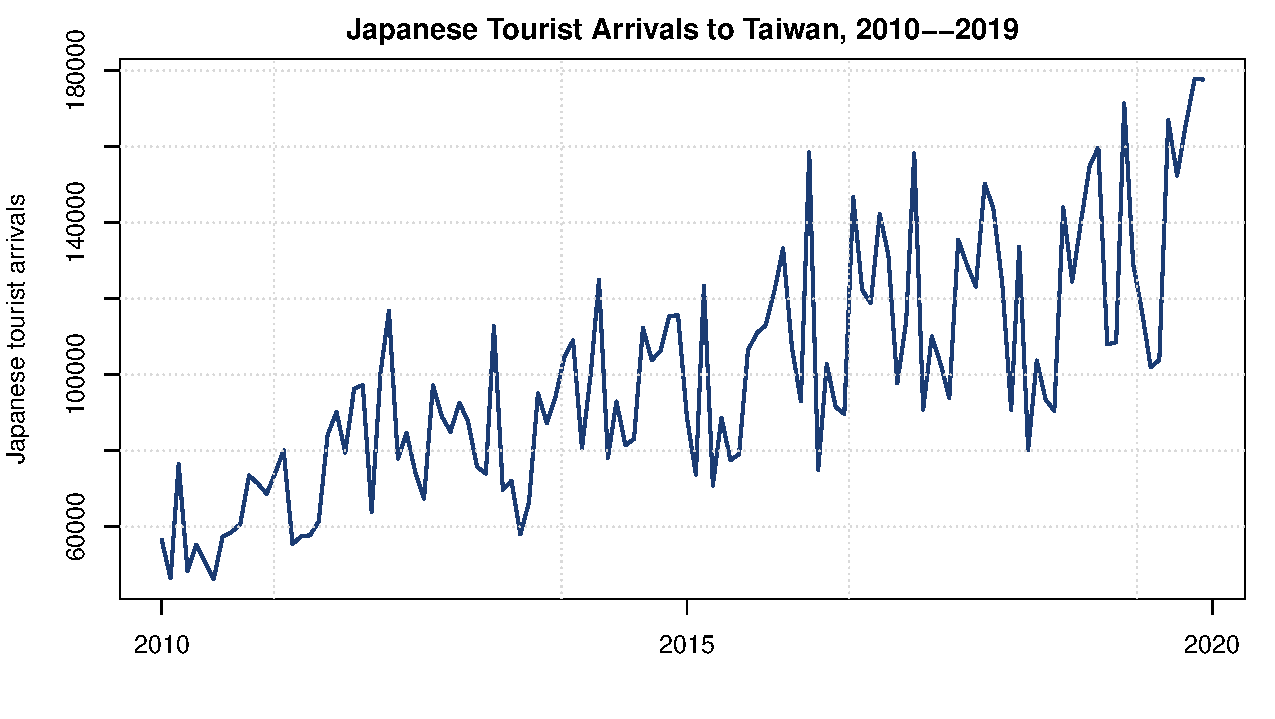
\includegraphics[width=0.91\textwidth,height=0.77\textheight,keepaspectratio]{figure1_tourist_trend.pdf}
\end{frame}

\begin{frame}{圖 1 告訴我們什麼？}
\begin{itemize}
  \item 日本來台觀光人數在 2010--2019 年之間呈現明顯上升趨勢。
  \item 這意味著若模型中沒有納入時間趨勢項，匯率或其他變數可能會錯誤吸收這個長期成長效果。
  \item 因此時間趨勢項不是裝飾，而是必要控制。
\end{itemize}
\end{frame}

\begin{frame}{圖 2：觀光需求季節性}
\centering
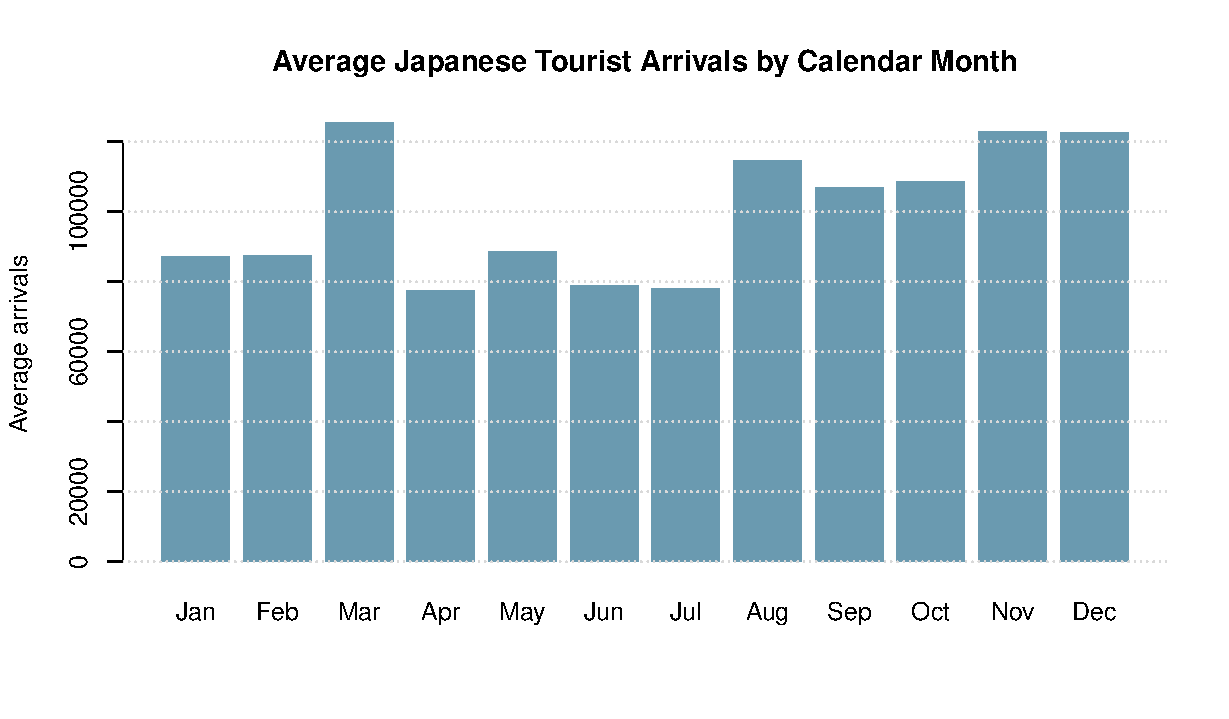
\includegraphics[width=0.88\textwidth,height=0.74\textheight,keepaspectratio]{figure2_seasonality.pdf}
\end{frame}

\begin{frame}{圖 2 告訴我們什麼？}
\begin{itemize}
  \item 不同月份的平均來台人數落差很大，顯示季節性相當強。
  \item 如果不控制月份效果，匯率或景氣變數的係數可能混入旺淡季差異。
  \item 這也是兩個模型都必須納入 Month dummies 的原因。
\end{itemize}
\end{frame}

\begin{frame}{描述性證據的重點}
\begin{columns}[T]
  \begin{column}{0.49\textwidth}
    \begin{block}{長期趨勢}
    \begin{itemize}
      \item 2010--2019 年間日人來台人數整體上升。
      \item 因此時間趨勢項具有明確經濟意義。
    \end{itemize}
    \end{block}
  \end{column}
  \begin{column}{0.49\textwidth}
    \begin{block}{季節性}
    \begin{itemize}
      \item 月份之間差異明顯。
      \item Month dummies 是必要解釋變數，不只是技術控制。
    \end{itemize}
    \end{block}
  \end{column}
\end{columns}
\end{frame}

\section{回歸結果}

\begin{frame}{主要回歸結果：核心係數}
\small
\begin{tabular}{lcccc}
\toprule
變數 & Model 1 & HAC $p$ & Model 2 & HAC $p$ \\
\midrule
$\Delta \ln(\mathrm{FX}_t)$ & -0.991 & 0.079 & -1.032 & 0.057 \\
$\ln(\mathrm{Tourist}_{t-1})$ & --- & --- & 0.505 & $<0.001$ \\
$\ln(\mathrm{JIPI}_t)$ & 0.302 & 0.583 & 0.840 & 0.011 \\
$\Delta \ln(\mathrm{OilPrice}_t)$ & -0.260 & 0.057 & -0.133 & 0.316 \\
Time trend & 0.007 & $<0.001$ & 0.003 & $<0.001$ \\
\bottomrule
\end{tabular}
\vspace{0.5em}
\begin{itemize}
  \item 匯率係數在兩個模型都為負，且都只有 10\% 水準邊際顯著。
  \item 動態模型中，落後一期旅客人數與當期 JIPI 顯著，代表需求慣性與景氣效果更穩定。
\end{itemize}
\end{frame}

\begin{frame}{先怎麼讀這張核心結果表？}
\begin{itemize}
  \item 第一欄是 Model 1，第二欄是 Model 2。
  \item 同一個變數在兩欄的比較，重點不只是係數大小，還包括顯著性是否改變。
  \item 若某個結果在兩個模型中方向一致，通常代表它比較穩定。
  \item 若加入動態項後結果明顯改變，則代表原本的靜態模型可能遺漏了重要的時間結構。
\end{itemize}
\end{frame}

\begin{frame}{Stata-style regression table（上）}
\small
\setlength{\tabcolsep}{4pt}
\begin{tabular}{lcc}
\toprule
Variable & (1) Static model & (2) Dynamic lag model \\
\midrule
$\Delta \ln(\mathrm{FX}_t)$ & -0.991* & -1.032* \\
 & (0.559) & (0.536) \\
$\Delta \ln(\mathrm{FX}_{t-1})$ & --- & 0.435 \\
 &  & (0.405) \\
$\Delta \ln(\mathrm{FX}_{t-2})$ & --- & -0.098 \\
 &  & (0.392) \\
$\ln(\mathrm{Tourist}_{t-1})$ & --- & 0.505*** \\
 &  & (0.082) \\
$\ln(\mathrm{JIPI}_t)$ & 0.302 & 0.840** \\
 & (0.548) & (0.323) \\
$\ln(\mathrm{JIPI}_{t-1})$ & --- & -0.623* \\
 &  & (0.373) \\
\bottomrule
\end{tabular}
\vspace{0.2em}

\scriptsize
HAC robust standard errors in parentheses. * $p<0.10$, ** $p<0.05$, *** $p<0.01$.
\end{frame}

\begin{frame}{Stata-style regression table（下）}
\small
\setlength{\tabcolsep}{4pt}
\begin{tabular}{lcc}
\toprule
Variable & (1) Static model & (2) Dynamic lag model \\
\midrule
$\ln(\mathrm{JIPI}_{t-2})$ & --- & 0.006 \\
 &  & (0.327) \\
$\Delta \ln(\mathrm{OilPrice}_t)$ & -0.260* & -0.133 \\
 & (0.135) & (0.132) \\
$\Delta \ln(\mathrm{OilPrice}_{t-1})$ & --- & 0.053 \\
 &  & (0.145) \\
$\Delta \ln(\mathrm{OilPrice}_{t-2})$ & --- & 0.116 \\
 &  & (0.129) \\
Time trend & 0.007*** & 0.003*** \\
 & (0.001) & (0.001) \\
Observations & 120 & 120 \\
Adjusted $R^2$ & 0.8805 & 0.9044 \\
\bottomrule
\end{tabular}
\vspace{0.2em}

\scriptsize
Month dummies are included in both models.
\end{frame}

\begin{frame}{Model 1：月份虛擬變數完整結果}
\scriptsize
\begin{tabular}{lccccc}
\toprule
月份 & 係數 & $p$ & 月份 & 係數 & $p$ \\
\midrule
1 月 & -0.223 & $<0.001$ & 7 月 & -0.392 & $<0.001$ \\
2 月 & -0.223 & 0.004 & 8 月 & 0.006 & 0.927 \\
3 月 & 0.089 & 0.080 & 9 月 & -0.097 & $<0.001$ \\
4 月 & -0.363 & $<0.001$ & 10 月 & -0.093 & $<0.001$ \\
5 月 & -0.225 & $<0.001$ & 11 月 & 0.005 & 0.778 \\
6 月 & -0.367 & $<0.001$ & 12 月 & 基準月 & --- \\
\bottomrule
\end{tabular}
\end{frame}

\begin{frame}{Model 1 的經濟解讀}
\begin{columns}[T]
  \begin{column}{0.49\textwidth}
    \begin{block}{經濟變數}
    \begin{itemize}
      \item 匯率：$-0.991$，方向與原始假說相反。
      \item 油價：$-0.260$，符合理論預期。
      \item JIPI：正向但不顯著。
    \end{itemize}
    \end{block}
  \end{column}
  \begin{column}{0.49\textwidth}
    \begin{block}{季節與趨勢}
    \begin{itemize}
      \item 4、6、7 月顯著低於 12 月。
      \item 3 月較高但只邊際顯著。
      \item 趨勢項高度顯著，代表長期需求成長。
    \end{itemize}
    \end{block}
  \end{column}
\end{columns}
\vspace{0.5em}
\begin{block}{油價係數的正確意義}
$\Delta \ln(\mathrm{OilPrice}_t)$ 是短期 semi-elasticity。若月油價成長率增加 0.01，來台人數約變動 $\beta_3$ 百分比；在 Model 1 中約為 $-0.260\%$。
\end{block}
\end{frame}

\begin{frame}{Model 1 結束後，我們得到什麼問題？}
\begin{itemize}
  \item 雖然 Model 1 已經抓到趨勢與季節性，但它仍把旅遊決策視為主要受當期資訊影響。
  \item 同時，若需求本身具有慣性，靜態模型可能會低估持續性帶來的影響。
  \item 因此下一步自然就是檢查：加入落後項之後，匯率與景氣效果會不會改變？
\end{itemize}
\end{frame}

\begin{frame}{Model 2：月份虛擬變數完整結果}
\scriptsize
\begin{tabular}{lccccc}
\toprule
月份 & 係數 & $p$ & 月份 & 係數 & $p$ \\
\midrule
1 月 & -0.158 & 0.001 & 7 月 & -0.208 & $<0.001$ \\
2 月 & -0.124 & 0.087 & 8 月 & 0.271 & $<0.001$ \\
3 月 & 0.164 & 0.001 & 9 月 & -0.136 & 0.004 \\
4 月 & -0.343 & $<0.001$ & 10 月 & -0.020 & 0.662 \\
5 月 & -0.017 & 0.760 & 11 月 & 0.065 & 0.026 \\
6 月 & -0.285 & $<0.001$ & 12 月 & 基準月 & --- \\
\bottomrule
\end{tabular}
\end{frame}

\begin{frame}{Model 2 的經濟解讀}
\begin{columns}[T]
  \begin{column}{0.49\textwidth}
    \begin{block}{核心結果}
    \begin{itemize}
      \item $\ln(\mathrm{Tourist}_{t-1})=0.505$，$p<0.001$。
      \item 表示觀光需求有明顯慣性與延續性。
      \item 當期 JIPI = 0.840，$p=0.011$。
    \end{itemize}
    \end{block}
  \end{column}
  \begin{column}{0.49\textwidth}
    \begin{block}{延遲效果}
    \begin{itemize}
      \item 落後匯率項不顯著。
      \item 落後油價項不顯著。
      \item 落後一期 JIPI 為負且僅邊際顯著，解讀應保守。
    \end{itemize}
    \end{block}
  \end{column}
\end{columns}
\vspace{0.5em}
\begin{itemize}
  \item 動態模型提高解釋力，但資料不支持很強的延遲匯率效果。
\end{itemize}
\end{frame}

\begin{frame}{Model 2 和 Model 1 相比，核心差異在哪裡？}
\begin{itemize}
  \item Model 2 最重要的新訊息，是落後一期旅客人數高度顯著。
  \item 這表示來台觀光人數不是每個月完全獨立決定，而是帶有強烈延續性。
  \item 一旦把這種持續性控制進來，JIPI 變得顯著，匯率則仍然維持負號但只邊際顯著。
  \item 換句話說，動態結構改變了我們對哪些變數更穩定的判斷。
\end{itemize}
\end{frame}

\begin{frame}{Actual vs Fitted}
\centering
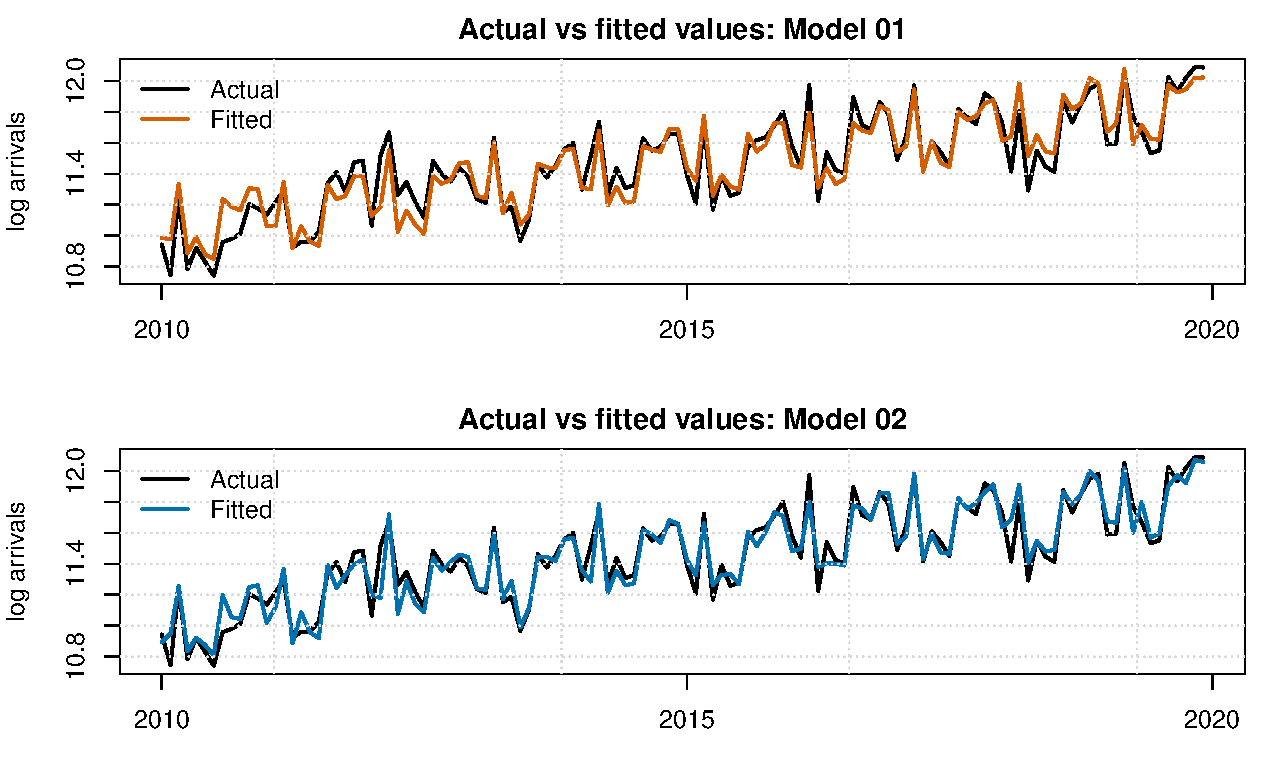
\includegraphics[width=0.90\textwidth,height=0.80\textheight,keepaspectratio]{figure3_actual_vs_fitted.pdf}
\end{frame}

\begin{frame}{兩個模型的綜合比較}
\begin{itemize}
  \item Model 2 的 adjusted $R^2$ 較高，配適表現優於 Model 1。
  \item 但兩個模型的共同結論一致：趨勢與季節性比匯率更穩定。
  \item 匯率係數在兩個模型中都為負，且都只有邊際顯著。
  \item 因此匯率重要，但不是最強的解釋來源。
\end{itemize}
\end{frame}

\section{穩健性與詮釋}

\begin{frame}{穩健性與診斷檢查}
\small
\begin{tabular}{lcc}
\toprule
檢查項目 & Model 1 & Model 2 \\
\midrule
F-statistic & 59.44 & 52.19 \\
F-test p-value & $<0.001$ & $<0.001$ \\
BG LM statistic & 27.982 & 16.114 \\
BG p-value & $<0.001$ & $<0.001$ \\
Maximum VIF & 3.27 & 9.75 \\
Adjusted $R^2$ & 0.8805 & 0.9044 \\
\bottomrule
\end{tabular}
\vspace{0.6em}
\begin{itemize}
  \item F 檢定顯示兩個模型整體上都顯著。
  \item BG 檢定顯示殘差仍有自相關，因此正式推論採 HAC 標準誤。
  \item Model 2 的最大 VIF 接近 10，表示引入落後項後共線性疑慮提高。
\end{itemize}
\end{frame}

\begin{frame}{負向匯率係數的可能解釋}
\begin{itemize}
  \item 替代效果：日圓升值也可能讓其他目的地更具吸引力。
  \item 避險效果：日圓升值可能伴隨全球不確定性上升。
  \item 遺漏變數：機票、航班供給、假期安排與競爭目的地價格未直接控制。
\end{itemize}
\end{frame}

\begin{frame}{研究限制與延伸方向}
\begin{columns}[T]
  \begin{column}{0.49\textwidth}
    \begin{block}{研究限制}
    \begin{itemize}
      \item 差分後的匯率與油價主要反映短期效果。
      \item 樣本期間侷限於 2010--2019。
      \item 仍存在殘差自相關與遺漏變數問題。
    \end{itemize}
    \end{block}
  \end{column}
  \begin{column}{0.49\textwidth}
    \begin{block}{延伸方向}
    \begin{itemize}
      \item 改用更長落後期間檢驗旅行規劃時差。
      \item 納入競爭目的地價格與航班供給資訊。
      \item 探討更完整的動態模型與結構變動。
    \end{itemize}
    \end{block}
  \end{column}
\end{columns}
\end{frame}

\section{結論}

\begin{frame}{結論}
\begin{enumerate}
  \item 匯率係數在兩個模型中都為負，且只有邊際顯著。
  \item 趨勢、季節性與落後一期旅客人數比匯率更穩定。
  \item JIPI 在動態模型中呈現正向且顯著效果。
  \item 因此不能把日圓升值直接解讀成日本來台人數必然上升。
\end{enumerate}
\end{frame}

\begin{frame}{政策意涵}
\begin{itemize}
  \item 不能假設日圓升值就會自然帶來更多日本旅客。
  \item 更重要的是台灣的相對吸引力、便利性與市場定位。
  \item 匯率是重要因素，但不是唯一因素。
\end{itemize}
\end{frame}

\begin{frame}{Q\&A}
  \vfill
  \centering
  {\Large 謝謝聆聽\par}
  \vspace{0.6em}
  {\large 歡迎提問\par}
  \vfill
\end{frame}

\end{document}
